\documentclass[11pt]{article}


% --- Packages ---
\usepackage{amsmath, amsthm, amsfonts, amssymb, hyperref, soul, latexsym, stmaryrd, booktabs} % fonts and characters
\usepackage{enumitem, ytableau, comment, graphicx, makecell, appendix, titling, scrextend, float, multirow, placeins, subcaption} % utilities
\usepackage{tikz, tikz-cd, tikzsymbols, pgfplots} % plots crap
\pgfplotsset{compat=1.18}
\usepackage{blkarray} % random math 
\usepackage{pstricks,pst-node,pst-tree} % networks
\usepackage{verbatim} % write code
\newlength\myverbindent % indent code
\setlength\myverbindent{0.5in} % change this to change indentation
\makeatletter
\def\verbatim@processline{%
  \hspace{\myverbindent}\the\verbatim@line\par}


% --- Matplotlib ---
% we import figures as pgfplots, which means its exported as tex to matplotlib
% to do this, we need certain commands in the premable to compile the way it shoud
\def\mathdefault#1{#1}
\everymath=\expandafter{\the\everymath\displaystyle}
\makeatletter\@ifpackageloaded{underscore}{}{\usepackage[strings]{underscore}}\makeatother


% --- Formatting ---
\usepackage{fullpage} % margins
\usepackage{setspace}
\doublespacing

\numberwithin{equation}{section} % number equations with section number
\numberwithin{figure}{section} % number figure with section number
\numberwithin{table}{section} % number table with section number


% --- Math Crap ---
\newcommand{\E}{\mathbb{E}}
\newcommand{\Z}{\mathbb{Z}}
\newcommand{\R}{\mathbb{R}}
\newcommand{\Q}{\mathbb{Q}}
\newcommand{\C}{\mathbb{C}}
\newcommand{\N}{\mathbb{N}}
\newcommand{\lagr}{\mathcal{L}}
\newcommand{\e}{\varepsilon}
\renewcommand{\sup}{\text{sup}}
\renewcommand{\inf}{\text{inf}}
\renewcommand{\d}{\delta}
\renewcommand{\Re}{\text{Re}}
\renewcommand{\Im}{\text{Im}}
\newcommand{\Arg}{\text{Arg}}
\newcommand{\Var}{\mathrm{Var}}
\newcommand{\Cov}{\mathrm{Cov}}


% --- Bibliography ---
\usepackage[style=numeric, backend=biber, ibidtracker=false]{biblatex} % packages
\bibliography{sources} % .bib file


% --- Title ---
\title{A Finite Element Approach to Reaction-Diffusion Systems}
\author{Gavin Engelstad\thanks{Replication code available at \url{https://github.com/GavinEngelstad/Reaction-Diffusion-FEM}.} \\ \href{mailto:gengelst@macalester.edu}{gengelst@macalester.edu}.}
\date{Fall 2024}


%% --- Document ---
\begin{document}

\maketitle

\begin{abstract}
    TBD
\end{abstract}


%% --- Paper Sections ---
% --- Introduction ---
\section{Introduction} \label{sec:intro}
Reaction-diffusion systems model the spatiotemporal behavior of various chemical and physical systems of one of more components that react with each other and diffuse across space. Chemical reactions \parencites{zhabotinsky2007belousov}{graham1993temperature}, the human nervous system \parencite{fitzhugh1961impulses}, population dynamics \parencite{clair2024reaction}, and the patterns that show up on animal's skins \parencites{turing1990chemical}{de2020leopard} can all be described using versions of a reaction-diffusion system. Within a system, reactions turn one substance into another as diffusion causes substances to spread out \parencite{li2020reaction}. The solutions to reaction-diffusion systems presents interesting patterns (dubbed ``Turing Patterns'' \parencite{vittadello2021turing}), moving fronts, and oscillations \parencites{szalai2004turing}{rinzel1982propagation}{turing1990chemical}.

Because of the wide range of applications reaction-diffusion systems have, it is important to have accurate and efficient computational methods to solve them. The main challenge to solving the reaction-diffusion systems is the nonlinear reaction term \parencites{pao1982nonlinear}{martin1992nonlinear}. This term drives the asymptotic behavior and stability of the system \parencite{pao1982nonlinear}, but it also introduces additional complexity, especially for methods that abuse local, linear approximations of the system to solve it. Finite differences \parencite{hoff1978stability}, spectral \parencites{bueno2014fourier}{craster2018spectral}, and analytic \parencites{spendier2013analytic} approaches can solve this problem with various degrees of computational efficiency and accuracy, but are limited to only work for certain reaction-diffusion systems or domain shapes.

This paper presents an approach to solving reaction-diffusion systems that uses the finite element method (FEM). The method in this paper is heavily based on the mathematical approach of \autocite{sellami2020accelerating} and \autocite{lang1992finite}. I utilize finite elements to discretize the space derivative and an implicit (backwards) Euler method to discretize the time derivative. Using a fine enough triangular mesh, the method is numerically stable and can be applied to a wide range of domains, including standard disks and rectangles, more complicated maze-like structures, and along the surface of 3D shapes.


% --- The Finite Element Method ---
\section{The Finite Element Method} \label{sec:fem}
\subsection{A General Reaction-Diffusion Equation and its Weak Form}

The general form of a reaction-diffusion system is
\[
    \partial_t \mathbf{u} = \Gamma \nabla^2 \mathbf{u} + \mathbf{R} (\mathbf{u})
\]
where $\mathbf{u}(t, x, y)$ is a vector function describing the concentration of the reactants, $\Gamma$ is a diagonal matrix of diffusion coefficients, and $\mathbf{R}(\mathbf{u})$ is a potential nonlinear function describing the reactions between the reactants \parencite{martin1992nonlinear}. I solve the system on the domain $\Omega$ and assume the PDE has Neumann boundary conditions with derivative 0 for simplicity. The method could be extended to Neumann conditions with nonzero gradient across the boundary or Dirichlet conditions, but this is beyond the scope of this paper. Assuming the systems contains $N$ total reactions, each equation in the system is
\[
    \partial_t u_n = \gamma_n \nabla^2 u_n + r_n\left(\{u_m\}_{m = 1}^{N}\right), \quad n \in \{1, 2, \dots, N\}.
\]

The FEM solves for a solution to the weak form of the PDE \parencite{galerkin1968rods}. The weak form is given by multiplying by some function $v$ and integrating across the whole domain, which gets
\[
    \int_\Omega v \partial_t u_n dA = \int_\Omega v \left[ \gamma_n \nabla^2 u_n + r_n\left(\{u_m\}_{m = 1}^{N}\right)\right] dA.
\]
By the product rule for gradients and Neumann boundary conditions, we know
\[
    \int_\Omega v \gamma_n \nabla^2 u_n = -\gamma_n \int_\Omega \nabla v \cdot \nabla u_n dA.
\]
Therefore, the weak form is
\[
    \int_\Omega v \partial_t u_n dA = -\gamma_n \int_\Omega \nabla v \cdot \nabla u_n dA + \int_\Omega v r_n\left(\{u_m\}_{m = 1}^{N}\right) dA.
\]


\subsection{Discretization}

\begin{figure}[t!]
    \centering
    \caption{Triangulations of different domains}

    \begin{subfigure}{\textwidth}
        \centering
        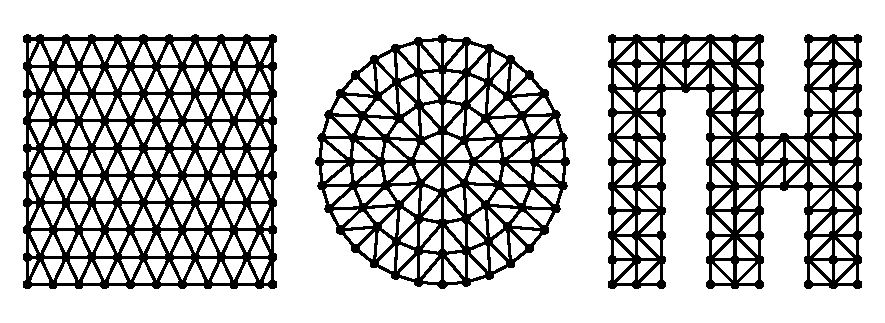
\includegraphics{figures/2dtris.pdf}
        \caption{2D Domains}
        \label{subfig:2dtris}
    \end{subfigure}

    \begin{subfigure}{\textwidth}
        \centering
        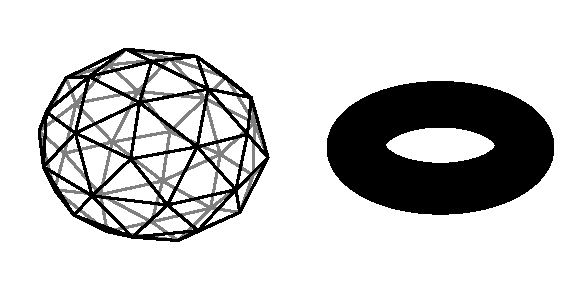
\includegraphics{figures/3dtris.pdf}
        \caption{3D Surface Domains}
        \label{subfig:3dtris}
    \end{subfigure}

    \label{fig:tris}
\end{figure}

To discretize the spacial derivative, I triangulate $\Omega$. Figure \ref{fig:tris} gives examples of what potential triangulations look like for a variety of domains. Panel \ref{subfig:2dtris} shows this discretization for 2D domains including a square, disk, and maze-like structure and Panel \ref{subfig:3dtris} shows this discretization along the surface of 3D objects, including a sphere and a torus.

For each vertex $v_i$ in the triangulation, I define a function $\psi_i$ such that
\begin{align*}
    \psi_i (v_i) &= 1 \\
    \psi_i (v_j) &= 0, \quad j \neq i
\end{align*}
and $\nabla \psi_i$ is constant along a triangle $T$. An example of $\psi_i$ for a vertex in the triangulation is in Figure \ref{fig:psi}. These functions will approximate the weak form of the PDE and the nonlinear reactions.

\begin{figure}[t!]
    \centering
    \caption{The function $\psi_i$ at a vertex}
    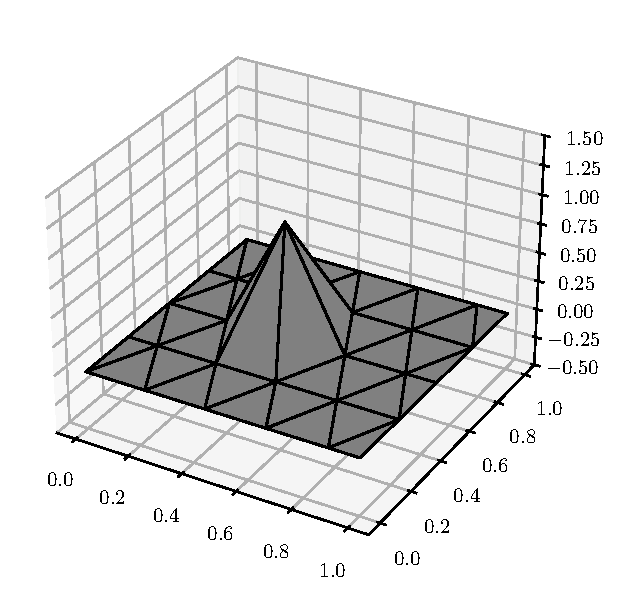
\includegraphics{figures/psi.pdf}
    \label{fig:psi}
\end{figure}

To discretize $u_n$, let $u_{n, i} (t)$ approximate $u(t, v_i)$. Then, we have
\[
    \hat{u}_n (t, x, y) = \sum_i \psi_i (x, y) u_{n, i} (t) \approx u(t, x, y).
\]
Similarly, we can approximate $r_n$ as
\[
    \hat{r}_n (t, x, y) = \sum_i \psi_i (x, y) r_n \left(\{u_{m, i} (t)\}_{m = 1}^N\right) \approx r_n(\{u_{m} (x, y, t)\}_{m = 1}^N).
\]
This approximation requires the solution for $u_n$ and $r_n$ to be adequately smooth across space and the triangulation to have a fine enough mesh. I analyze these assumptions in Section \ref{subsec:err} by solving systems with increasingly fine discretizations to get closer to the exact answer. Using these approximations and $v = \psi_i$ in the weak form gets
\[
    \sum_j \partial_t u_{n, j} \int_\Omega \psi_i \psi_j dA = -\gamma_n \sum_j u_{n, j} \int_\Omega \nabla \psi_i \cdot \nabla \psi_j dA + \sum_j r_n \left(\{u_{m, j} (t)\}_{m = 1}^N\right) \int_\Omega \psi_i \psi_j dA
\]
which represents the spatially discretized version of the system.

The temporal discretization is chosen to handle potential nonlinearities in the reaction function as well as maximize numerical stability. Specifically, I combine an explicit (forwards) Euler method to discretize the reaction step and an implicit (backwards) Euler method to discretize the diffusion step \parencite{sellami2020accelerating}. The explicit Euler step evaluates the reaction with known quantities to hangle nonlinearities before setting up a linear system, and the implicit Euler step maximizes the numerical stability of the solution \parencite{folland2020introduction}. Letting $u_{n, i}^t = u_{n, i}(t)$ at some discrete time step $t$, the time-discretized equation is
\[
    \sum_j u_{n, j}^t \left(\int_\Omega \psi_i \psi_j dA + \Delta t \gamma_n \int_\Omega \nabla \psi_i \cdot \nabla \psi_j dA\right) = \sum_j \left(u_{n, j}^{t - \Delta t} + \Delta t r_n \left(\{u_{m, j}^{t - \Delta t}\}_{m = 1}^N\right)\right) \int_\Omega \psi_i \psi_j dA.
\]


\subsection{Setting up a Linear System}

To solve the time-discretized equation, I turn it into a linear algebra problem. I define the damping matrix $\mathbf{D}$ so that
\[
    d_{i, j} = \int_\Omega \psi_i \psi_j dA
\]
and the stiffness matrix $\mathbf{S}$ so that
\[
    s_{i, j} = \int_\Omega \nabla \psi_i \cdot \nabla \psi_j dA.
\]
Since $d_{i, j} = 0$ and $s_{i, j} = 0$ whenever $v_i$ and $v_j$ don't share a triangle, the damping and stiffness matrices have a sparse structure that makes computation with them fast even on very fine triangulations of $\Omega$. Appendix \ref{app:mats} derives expressions for $d_{i, j}$ and $s_{i, j}$ in cases where $v_i$ and $v_j$ share at least one triangle.

Then, defining $\mathbf{u}_n^t$ as the vector with entries $u_{n, j}^t$, the equation becomes the linear system
\[
    \left(\mathbf{D} + \Delta t \gamma_n \mathbf{S}\right) \mathbf{u}_n^t = \mathbf{D} \left(\mathbf{u}_n^{t - \Delta t} + \Delta t r_n \left(\{\mathbf{u}_m^{t - \Delta t}\}_{m = 1}^N\right)\right)
\]
which allows me to solve for the solution at $t$ given a solution at time $t - \Delta t$. The function $r_n$ is vectorized and because $\mathbf{D} + \Delta t \gamma_n \mathbf{S}$ is sparse, symmetric, and positive-definite, I use the conjugate gradient method to solve for $\mathbf{u}_n^t$ \parencite{nazareth2009conjugate}. Together, this allows me to quickly solve for each time step.

Therefore, to solve the system I start with some initial condition $\mathbf{u}_n^0$ for each $n$. In the sections that follow, this initial condition is chosen to be random noise, although any initial condition could be used. Then, I solve the linearized version of the PDE for each $n$ to iterate to the next time step. Repeating this process to some final $T$ allows me to efficiently and accurately solve the reaction-diffusion PDE on any triangulated domain.



% --- Simple Solutions ---
\section{Solving a System} \label{sec:sols}
\subsection{A Baseline System}

For this paper, I solve the system in \autocites{othmer2009intersection}{jeong2017numerical}. By replacing the reaction function, the method can be extended to any sufficiently smooth reaction diffusion system. This includes Turing's initial version \parencites{turing1990chemical}{de2020leopard} and other activator-inhibitor equations \parencites{landge2020pattern}{meinhardt2000pattern} which it has been tested against. The system I solve is given by
\begin{align*}
    \frac{\partial u}{\partial t} = \gamma_u \nabla^2 u + k_1 \left(v - \frac{uv}{1 + v^2}\right) \\
    \frac{\partial v}{\partial t} = \gamma_v \nabla^2 v + k_2 - v - \frac{4 u v}{1 + v^2}.
\end{align*}

Like \autocite{jeong2017numerical}, I fix $D_u = 1$ and $k_2 = 11$ in all simulations. I vary $D_v$ and $k_1$ across simulations to create different Turning patterns, but we always have $D_v< D_u$. The time step is set to $\Delta t = 0.01$, and all systems are iterated until $t = 1,000$, at which point they all have reached a steady state. I triangulate so that there are 250 points per square unit of the domain I solve the PDE on. The plotted solutions will be of $u$, although $v$ makes a similar pattern.


\subsection{Solutions}

\begin{figure}[t!]
    \centering
    \caption{Solutions to the reaction diffusion system}

    \begin{subfigure}{\textwidth}
        \centering
        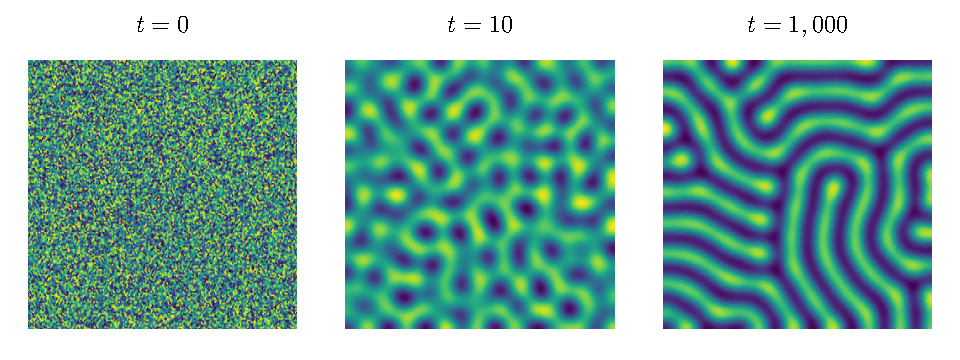
\includegraphics{figures/square_ts.pdf}
        \caption{$10 \times 10$ square domain}
    \end{subfigure}

    \begin{subfigure}{\textwidth}
        \centering
        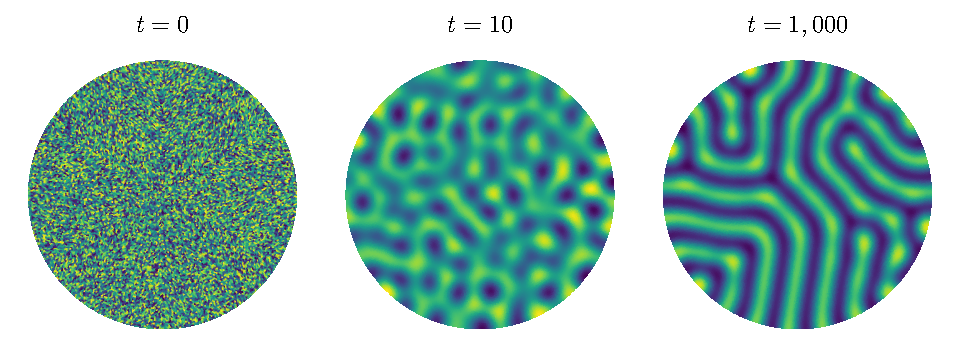
\includegraphics{figures/circle_ts.pdf}
        \caption{Radius 5 circular domain}
    \end{subfigure}
    \label{fig:sol-ts}
\end{figure}

Figure \ref{fig:sol-ts} plots the solution to the reaction diffusion system at different time steps on a square and circular domain. The left panel plots the initial condition, the middle panel plots an intermediate step during the reaction, and the right panel plots the system at steady state. I set the initial condition to random noise. At $t = 10$, the reaction starts to progress, and we see patterns and `hotspots' emerge. The patterns that exist, however, lack clear definition. In the steady state, we see well-defined lines that form clear Turing patterns.

At each time step, the system makes similar shapes on the circular and square domains. The intermediate step patterns both have similarly sized hotspots, and the Turing patterns that develop have a similar structure being made of curved-lines with similar width. I explore this further in Section \ref{sec:doms} with more complicated domains and arrive at the same result.


\subsection{Parameters}

\begin{figure}[t!]
    \centering
    \caption{$10 \times 10$ square steady states for different $\gamma_v$ and $k_1$}
    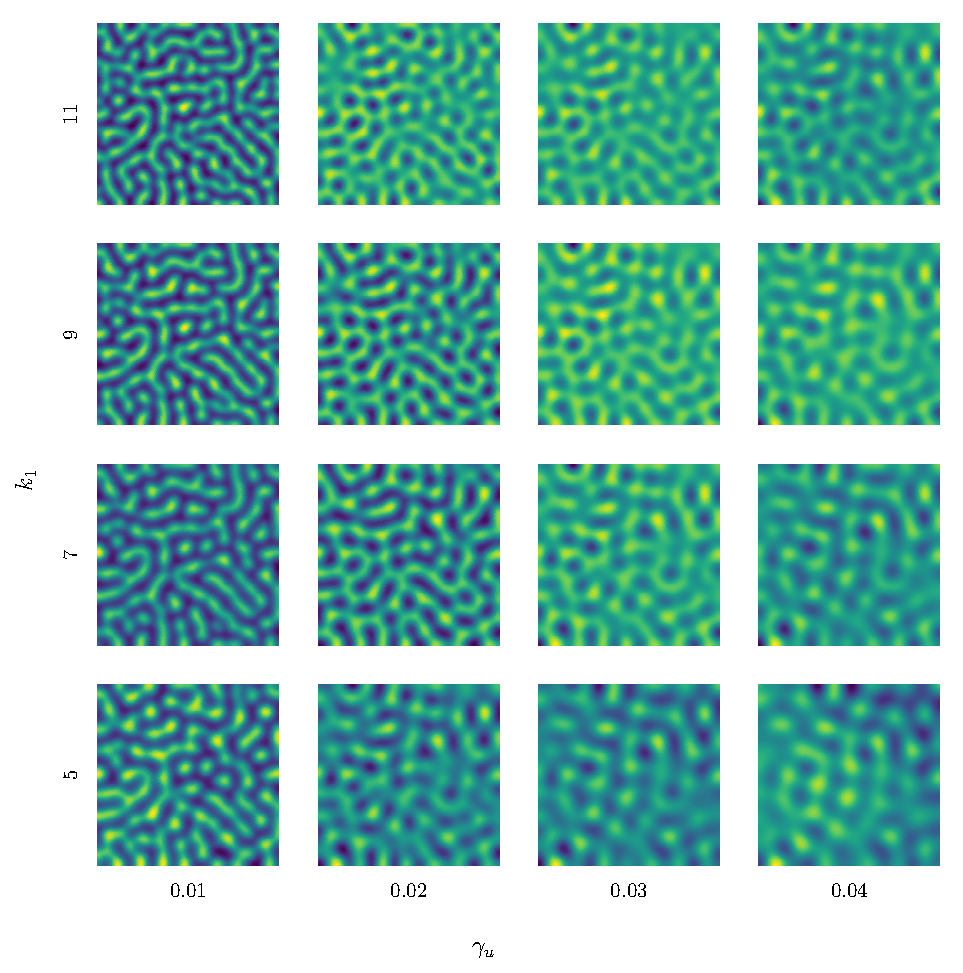
\includegraphics{figures/square_params.pdf}
    \label{fig:sq-pars}
\end{figure}

\begin{figure}[t!]
    \centering
    \caption{Radius 5 circle steady states for different $\gamma_v$ and $k_1$}
    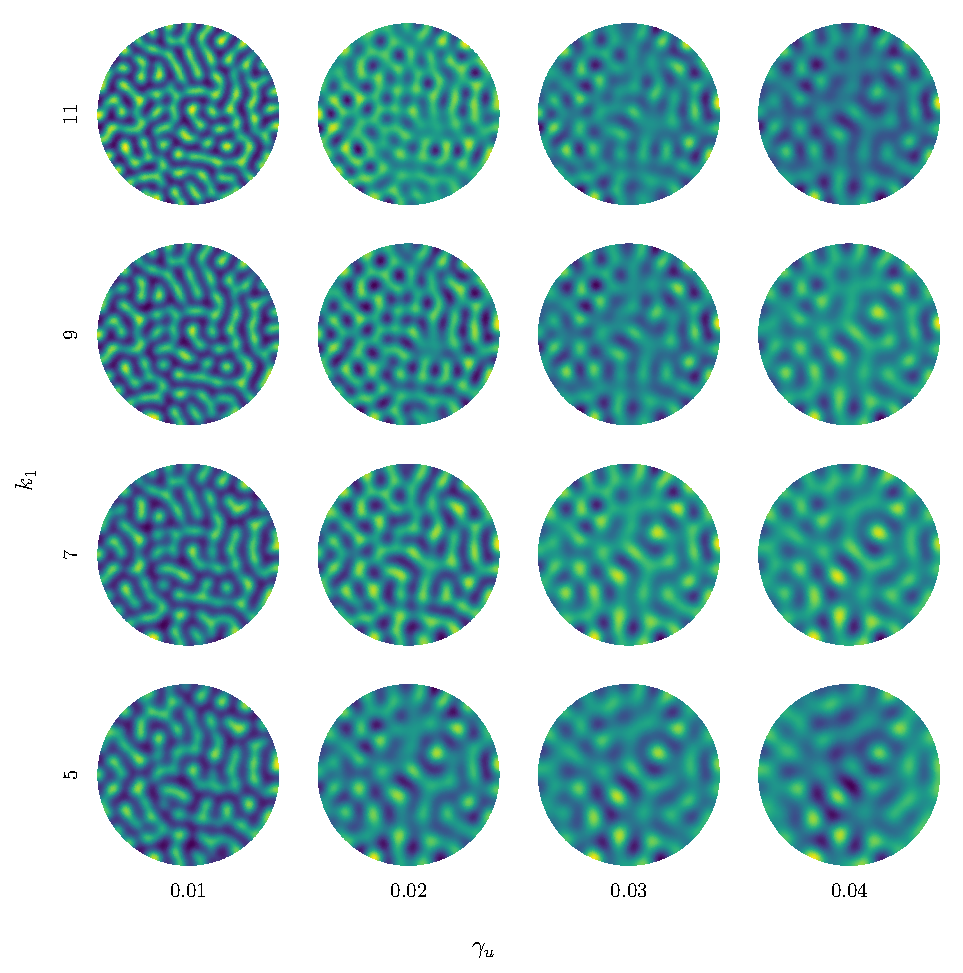
\includegraphics{figures/circle_params.pdf}
    \label{fig:cir-pars}
\end{figure}













% --- Complex Domains ---
\section{More Complex Domains} \label{sec:doms}
% maze
% 3d surface



%% --- References ---
\newpage
\printbibliography
\FloatBarrier


%$ --- Appendix ---
\newpage
\appendix

% --- Dtiffness and Dapening Matricies ---
\section{The Stiffness and Damping Matrices} \label{app:mats}
\subsection{The Area of a Triangle}

Given a triangle $T$ with corners $(x_i, y_i, z_i)$, $(x_j, y_j, z_j)$, and $(x_k, y_k, z_k)$, the area of the triangle $A_T$ is
\[
    A_T = \frac{1}{2} \left| \begin{pmatrix}
        x_j - x_i \\ y_j - y_i \\ z_j - z_i
    \end{pmatrix} \times \begin{pmatrix}
        x_k - x_i \\ y_k - y_i \\ z_k - z_i
    \end{pmatrix} \right| = \frac{1}{2} \begin{vmatrix}
        (y_j - y_i)(z_k - z_i) - (y_k - y_i)(z_j - z_i) \\
        (x_k - x_i)(z_j - z_i) - (x_j - x_i)(z_k - z_i) \\
        (x_j - x_i)(y_k - y_i) - (x_k - x_i)(y_j - y_i)
    \end{vmatrix}.
\]

In the 2D case where $z_i = z_j = z_k$, this becomes\footnote{Technically, this could be the negative of the area and to get the actual area you need to take an absolute value. Solving it this way makes the next steps easier, however.}
\[
    A_T = \frac{1}{2} \left[(x_j - x_i)(y_k - y_i) - (x_k - x_i)(y_j - y_i)\right] = \frac{1}{2} \left(x_i y_j + x_j y_k + x_k y_i - x_i y_k - x_k y_j - x_j y_i\right).
\]

\subsection{The Damping Matrix}

The damping matrix $\mathbf{D}$ is defined so that
\[
    d_{i, j} = \int_\Omega \psi_i \psi_j dA.
\]
I consider a triangle $T$ with both $v_i$ and $v_j$ as vertices to $T$. From the solution for $T$, we know
\[
    d_{i, j} = \sum_{\{T: v_i, v_j \in T\}} \int_T \psi_i \psi_j dA.
\]

\begin{figure}[t!]
    \centering
    \caption{Transformation from $T^0$ to $T$.}

    \begin{subfigure}{0.27\textwidth}
        \resizebox{\textwidth}{!}{%
        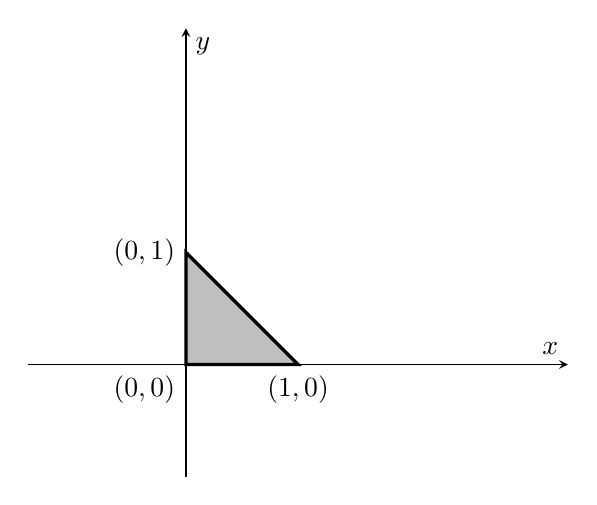
\begin{tikzpicture}
            \begin{axis}[xlabel=$x$, ylabel=$y$, axis lines=middle, xtick={6}, ytick={6}, no marks, axis equal, xmin=-1, xmax=3, ymin=-1, ymax=3]
                \draw[very thick, fill=lightgray] (0,0) node[anchor=north east]{$(0, 0)$}
                -- (1,0) node[anchor=north]{$(1, 0)$}
                -- (0,1) node[anchor=east]{$(0, 1)$}
                -- cycle;
            \end{axis}
        \end{tikzpicture}%
        }
        \caption{Initial triangle $T^0$}%
    \end{subfigure} \quad
    \begin{subfigure}{0.27\textwidth}%
        \resizebox{\textwidth}{!}{%
        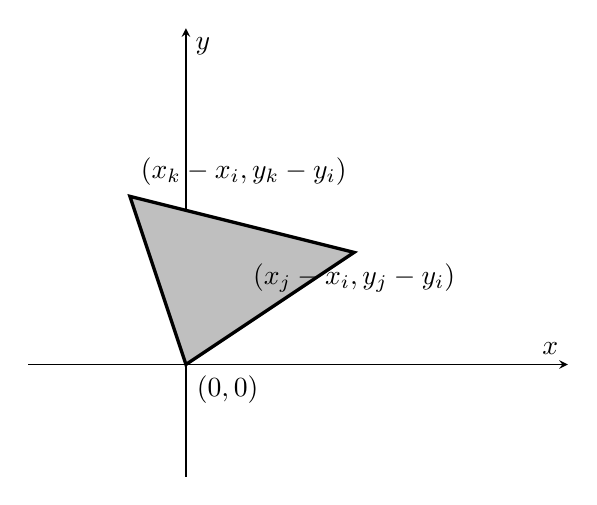
\begin{tikzpicture}
            \begin{axis}[xlabel=$x$, ylabel=$y$, axis lines=middle, xtick={6}, ytick={6}, no marks, axis equal, xmin=-1, xmax=3, ymin=-1, ymax=3]
                \draw[very thick, fill=lightgray] (0,0) node[anchor=north west]{$(0, 0)$}
                -- (1.5,1) node[anchor=north]{$(x_j - x_i, y_j - y_i)$}
                -- (-0.5,1.5) node[anchor=south west]{$(x_k - x_i, y_k - y_i)$}
                -- cycle;
            \end{axis}
        \end{tikzpicture}%
        }
        \caption{Rotated and scaled}%
    \end{subfigure} \quad
    \begin{subfigure}{0.27\textwidth}%
        \resizebox{\textwidth}{!}{%
        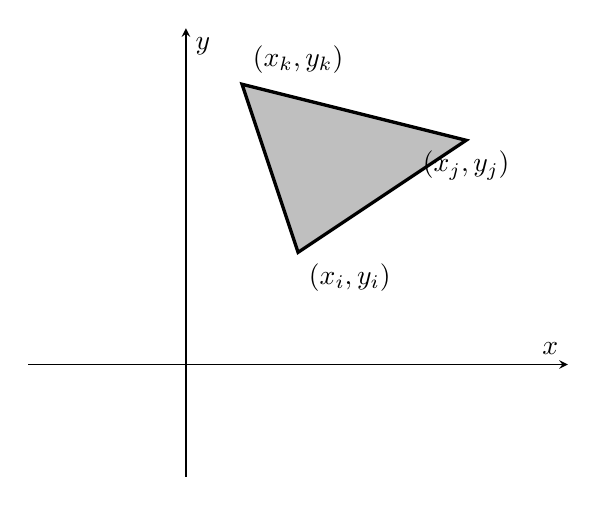
\begin{tikzpicture}
            \begin{axis}[xlabel=$x$, ylabel=$y$, axis lines=middle, xtick={6}, ytick={6}, no marks, axis equal, xmin=-1, xmax=3, ymin=-1, ymax=3]
                \draw[very thick, fill=lightgray] (1,1) node[anchor=north west]{$(x_i, y_i)$}
                -- (2.5,2) node[anchor=north]{$(x_j, y_j)$}
                -- (0.5,2.5) node[anchor=south west]{$(x_k, y_k)$}
                -- cycle;
            \end{axis}
        \end{tikzpicture}%
        }
        \caption{Translated to $T$}
    \end{subfigure}

    \label{fig:T0-to-T}
\end{figure}

To calculate this integral over $T$, we will first define an affine transformation from $T^0$ to $T$ where $T^0$ is a right triangle with $v_i = (0, 0)$, $v_j = (1, 0)$, and $v_k = (0, 1)$ (Figure \ref{fig:T0-to-T}). To map from $\tilde{x}, \tilde{y}$ on $T^0$ to $T$, we first scale and rotate according to the linear transformation
\[
    \begin{pmatrix}
        x_j - x_i & x_k - x_i \\
        y_j - y_i & y_k - y_i \\
    \end{pmatrix} \begin{pmatrix}
        \tilde{x} \\ \tilde{y}
    \end{pmatrix}
\]
then add $(x_i, y_i)^\top$ to get to $T$. Therefore, to get from $\tilde{x}, \tilde{y}$ on $T^0$ to $x, y$ on $T$, we use
\begin{align*}
    x = x_i + (x_j - x_i) \tilde{x} + (x_k - x_i) \tilde{y} \\
    y = y_i + (y_j - y_i) \tilde{x} + (y_k - y_i) \tilde{y}.
\end{align*}
The Jacobian of this transformation
\[
    \begin{pmatrix}
        x_j - x_i & x_k - x_i \\
        y_j - y_i & y_k - y_i
    \end{pmatrix}
\]
has determinant
\[
    \begin{vmatrix}
        x_j - x_i & x_k - x_i \\
        y_j - y_i & y_k - y_i
    \end{vmatrix} = (x_j - x_i)(y_k - y_i) - (x_k - x_i)(y_j - y_i) = 2 A_T.
\]
Therefore, we get
\[
    \int_T \psi_i(x, y) \psi_j(x, y) dydx = 2 A_t \int_{T^0} \psi_i(\tilde{x}, \tilde{y}) \psi_j(\tilde{x}, \tilde{y}) d\tilde{y}d\tilde{x}x.
\]

On $T^0$, we have
\[
    \psi_i (\tilde{x}, \tilde{y}) = 1 - \tilde{x} - \tilde{y} \quad \text{and} \quad \psi_j (\tilde{x}, \tilde{y}) = \tilde{x}.
\]
Therefore, we know
\begin{align*}
    \int_T \psi_i(x, y) \psi_i(x, y) dydx &= 2 A_T \int_{T^0} \psi_i(\tilde{x}, \tilde{y}) \psi_i(\tilde{x}, \tilde{y}) d\tilde{y}d\tilde{x} \\
    &= 2 A_T \int_0^1 \int_0^{1 - \tilde{x}} (1 - \tilde{x} - \tilde{y})^2 d\tilde{y}d\tilde{x} \\
    &= 2 A_T \int_0^1 \int_0^{1 - \tilde{x}} \left[ 1 - 2 \tilde{x} - 2 \tilde{y} + 2 \tilde{x} \tilde{y} + \tilde{x}^2 + \tilde{y}^2 \right] d\tilde{y}d\tilde{x} \\
    &= \frac{2}{3} A_T \int_0^1 (1 - \tilde{x})^3 d\tilde{x} \\
    &= \frac{2}{3} A_T \int_1^0 \hat{x}^3 (-1) d\hat{x}, \quad \hat{x} = 1 - \tilde{x} \\
    &= \frac{1}{6} A_T
\end{align*}
and
\begin{align*}
    \int_T \psi_I(x, y) \psi_j(x, y) dydx &= 2 A_T \int_{T^0} \psi_i(\tilde{x}, \tilde{y}) \psi_j(\tilde{x}, \tilde{y}) d\tilde{y}d\tilde{x} \\
    &= 2 A_T \int_0^1 \int_0^{1 - \tilde{x}} (1 - \tilde{x} - \tilde{y}) \tilde{x} d\tilde{y}d\tilde{x} \\
    &= 2 A_T \int_0^1 \tilde{x} \int_0^{1 - \tilde{x}} (1 - \tilde{x} - \tilde{y}) d\tilde{y}d\tilde{x} \\
    &= A_T \int_0^1 \tilde{x} (1 - \tilde{x})^2 d\tilde{x} \\
    &= A_T \int_1^0 (\hat{x}^2 - \hat{x}^3) (-1) d \hat{x}, \quad \hat{x} = 1 - \tilde{x} \\
    &= \frac{1}{12} A_T.
\end{align*}

Along a 3D surface, the same equation holds. We use the transformation
\begin{align*}
    x = x_i + (x_j - x_i) \tilde{x} + (x_k - x_i) \tilde{y} \\
    y = y_i + (y_j - y_i) \tilde{x} + (y_k - y_i) \tilde{y} \\
    z = z_i + (z_j - z_i) \tilde{x} + (z_k - z_i) \tilde{y}
\end{align*}
and the fact that the change in area elements is the ratio of the areas
\[
    \frac{A_T}{A_{T^0}} = \frac{A_T}{\frac{1}{2}} = 2 A_T
\]
to get to the same result.


\subsection{The Stiffness Matrix}

The stiffness matrix $\mathbf{S}$ is defined so that
\[
    s_{i, j} = \int_\Omega \nabla \psi_i \cdot \nabla \psi_j dA.
\]
Like with the damping matrix, I will calculate the integral over a single triangle $T$. Then, we can calculate
\[
    s_{i, j} = \sum_{\{T: v_i, v_j \in T\}} \int_T \nabla \psi_i \cdot \nabla \psi_j dA.
\]

\begin{figure}[t!]
    \centering
    \caption{$\vec{w}$ on a triangle}
    \begin{tikzpicture}
        \draw[darkgray] (0,0) node[anchor=east]{$v_i$}
            -- (2,-4) node[anchor=north]{$v_j$}
            -- (5,-1) node[anchor=west]{$v_k$}
            -- cycle;

        \draw[Stealth-, thick] (0,0) -- node[above] {$\vec{w}$} ++ (3,-3);
    \end{tikzpicture}
    \label{fig:grad-psi}
\end{figure}

To calculate the integral over $T$, recognize $\nabla \psi_i$ is constant over $T$. Therefore, we know
\[
    \int_T \nabla \psi_i \cdot \nabla \psi_j dA = A_T \nabla \psi_i \cdot \nabla \psi_j.
\]
We know $\nabla \psi_i$ is a vector pointing into $v_i$ orthogonal to $v_j - v_k$. Defining $\vec{w}$ to be orthogonal to $v_j - v_k$ such that
\[
    v_i - v_j = \lambda (v_j - v_k) + \vec{w}
\]
for some scalar $\lambda$, we know
\[
    \vec{w} = v_i - v_j - \frac{(v_i - v_j) \cdot (v_j - v_k)}{(v_j - v_k) \cdot (v_j - v_k)} (v_j - v_k).
\]
An example of this is given in Figure \ref{fig:grad-psi}. Then, we know $\frac{1}{|\vec{w}|}$ is the magnitude of the gradient\footnote{Shoutout $
\frac{\text{rise}}{\text{run}}$.} and $\frac{1}{|\vec{w}|} \vec{w}$ is the direction of the gradient. Therefore, the gradient is
\[
    \nabla \psi_i = \frac{1}{|\vec{w}|^2} \vec{w}.
\]

In the 3D surface case, I directly implement this formula to calculate the stiffness matrix. In the 2D case, the $\vec{w}$ vector is
\begin{align*}
    \vec{w} &= \begin{pmatrix}
        x_i - x_j \\ y_i - y_j
    \end{pmatrix} - \frac{(x_i - x_j)(x_j - x_k) + (y_i - y_j)(y_j - y_k)}{(x_j - x_k)^2 + (y_j - y_k)^2} \begin{pmatrix}
        x_j - x_k \\ y_j - y_k
    \end{pmatrix} \\
    &= \frac{1}{(x_j - x_k)^2 + (y_j - y_k)^2} \begin{pmatrix}
        (x_i - x_j) (y_j - y_k)^2 - (x_j - x_k) (y_i - y_j) (y_j - y_k) \\
        (x_j - x_k)^2 (y_i - y_j) - (x_i - x_j)(x_j - x_k) (y_j - y_k)
    \end{pmatrix} \\
    &= \frac{(x_i - x_j)(y_j - y_k) - (x_j - x_k) (y_i - y_j)}{(x_j - x_k)^2 + (y_j - y_k)^2} \begin{pmatrix}
        y_j - y_k \\ x_k - x_j
    \end{pmatrix} \\
    &= \frac{x_i y_j + x_j y_k + x_k y_i - x_i y_k - x_k y_j - x_j y_i}{(x_j - x_k)^2 + (y_j - y_k)^2} \begin{pmatrix}
        y_j - y_k \\ x_k - x_j
    \end{pmatrix} \\
    &= \frac{2 A_T}{(x_j - x_k)^2 + (y_j - y_k)^2} \begin{pmatrix}
        y_j - y_k \\ x_k - x_j.
    \end{pmatrix}
\end{align*}
Then, the gradient is
\begin{align*}
    \nabla \psi_i &= \frac{1}{|\vec{w}|^2} \vec{w} \\
    &= \frac{(x_j - x_k)^2 + (y_j - y_k)^2}{2 A_T} \left(\begin{pmatrix}
        y_j - y_k \\ x_k - x_j
    \end{pmatrix} \cdot \begin{pmatrix}
        y_j - y_k \\ x_k - x_j
    \end{pmatrix}\right)^{-1} \begin{pmatrix}
        y_j - y_k \\ x_k - x_j
    \end{pmatrix} \\
    &= \frac{1}{2 A_T} \begin{pmatrix}
        y_j - y_k \\ x_k - x_j
    \end{pmatrix}.
\end{align*}

This means the integrals over the gradients become
\[
    \int_T \nabla \psi_i \cdot \nabla \psi_i dA = \frac{1}{4 A_T} \left((y_j - y_k)^2 + (x_k - x_j)^2\right)
\]
and
\[
    \int_T \nabla \psi_i \cdot \nabla \psi_i dA = \frac{1}{4 A_T} \left((y_j - y_k)(y_k - y_i) + (x_k - x_j)(x_i - x_k)\right)
\]
which I plug into the stiffness matrix.




\end{document}
